\subsection*{counter with scan chain}


\begin{figure}[H]
\centering
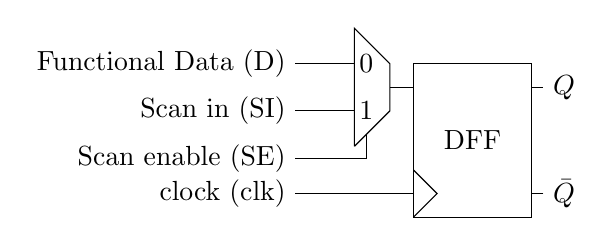
\begin{tikzpicture}[scale=1.2]

%DFF
\draw  (-1.25,1) rectangle (0,-0.625) node[pos=.5]{DFF};
\draw (-1.25,-0.125) -- (-1,-0.375) -- (-1.25,-0.625);

%MUX
\draw
(-1.875,0.125) -- 
(-1.5,0.5) -- 
(-1.5,1) -- 
(-1.875,1.375) --
(-1.875,0.125);
\node at (-1.75,1) {0};
\node at (-1.75,0.5) {1};

% connection
\draw (-1.5,0.75) -- (-1.25,0.75);
 
% inputs
\draw (-2.5,-0.375) -- (-1.25,-0.375);
\node [anchor=east] at (-2.5,-0.375) {clock (clk)};
\draw(-1.875,1) -- (-2.5,1);
\node [anchor=east] at (-2.5,1) {Functional Data (D)};
\draw(-1.875,0.5) -- (-2.5,0.5);
\node [anchor=east] at (-2.5,0.5) {Scan in (SI)};
\draw (-1.75,0.25) |- (-2.5,0);
\node [anchor=east] at (-2.5,0) {Scan enable (SE)};

%ouputs
\draw (0,0.75) -- (0.125,0.75);
\node [anchor=west] at (0.125,0.75) {$Q$};
\draw(0.125,-0.375) -- (0,-0.375);
\node [anchor=west] at (0.125,-0.375) {$\bar{Q}$};
\draw (-1.75,0.25) |- (-2.5,0);


\end{tikzpicture}
\caption{Scan Flipflop (SFF)}
\label{tkz:SFF}
\end{figure}

\begin{figure}[H]
\centering
\tikzstyle{dot} = [draw,shape=circle,fill=black, scale =.2]
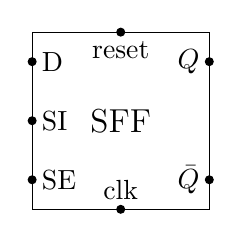
\begin{tikzpicture}[scale=1.5]

\draw  (-2.5,1) rectangle (-1,-0.5) node[pos=.5]{\large{SFF}};
\node [anchor=west] at (-2.5,0.75) {D};
\node [anchor=west] at (-2.5,0.25) {SI};
\node [anchor=west] at (-2.5,-0.25) {SE};
\node [anchor=east] at (-1,0.75) {$Q$};
\node [anchor=east] at (-1,-0.25) {$\bar{Q}$};
\node [anchor=south] at (-1.75,-0.5) {clk};
\node [anchor=north] at (-1.75,1) {reset};

\node [dot] at (-2.5,0.75) {};
\node [dot] at (-1.75,1) {};
\node [dot] at (-2.5,0.25) {};
\node [dot] at (-2.5,-0.25) {};
\node [dot] at (-1.75,-0.5) {};
\node [dot] at (-1,-0.25) {};
\node [dot] at (-1,0.75) {};

%\node [anchor=south] at (-1.75,1) {SFF};
\end{tikzpicture}
\caption{Symbol Scan Flipflop (SFF)}
\label{tkz:SFFSymbol}
\end{figure}

\begin{figure}[H]
\centering
\tikzstyle{dot} = [draw,shape=circle,fill=black, scale =.2]
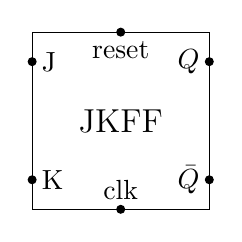
\begin{tikzpicture}[scale=1.5]

\draw  (-2.5,1) rectangle (-1,-0.5)node[pos=.5]{\large{JKFF}};
\node [anchor=west] at (-2.5,0.75) {J};
\node [anchor=north] at (-1.75,1) {reset};
\node [anchor=west] at (-2.5,-0.25) {K};
\node [anchor=east] at (-1,0.75) {$Q$};
\node [anchor=east] at (-1,-0.25) {$\bar{Q}$};
\node [anchor=south] at (-1.75,-0.5) {clk};

\node [dot] at (-2.5,0.75) {};
\node [dot] at (-1.75,1) {};
\node [dot] at (-2.5,-0.25) {};
\node [dot] at (-1.75,-0.5) {};
\node [dot] at (-1,-0.25) {};
\node [dot] at (-1,0.75) {};

\end{tikzpicture}
\caption{Symbol JK-Flipflop (JKFF)}
\label{tkz:JKFFSymbol}
\end{figure}

\begin{figure}[H]
\centering
\tikzstyle{dot} = [draw,shape=circle,fill=black, scale =.3]
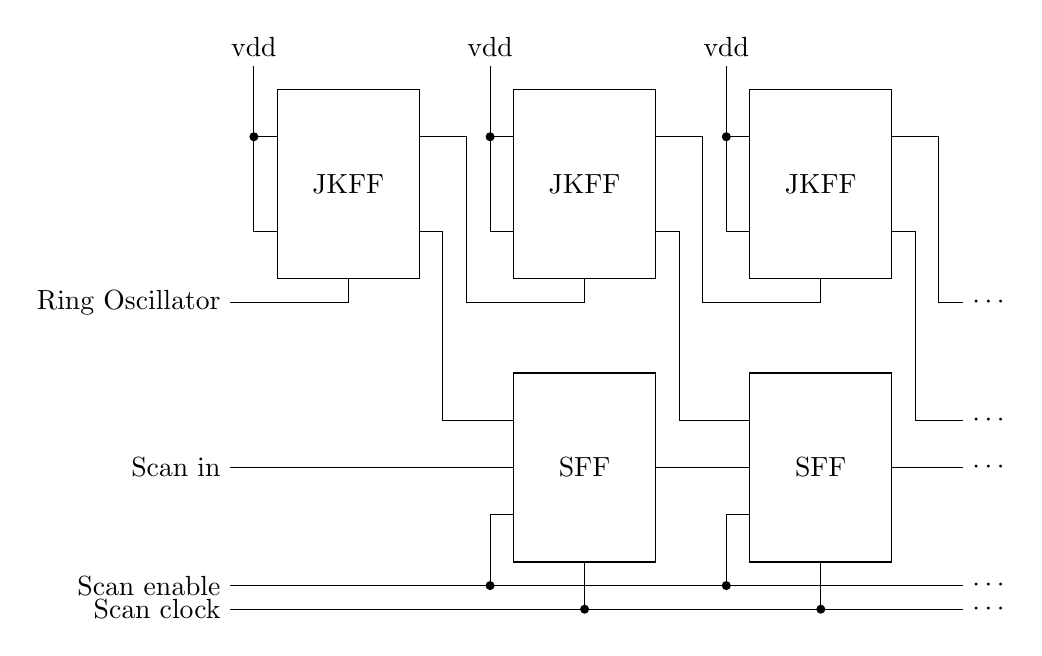
\begin{tikzpicture}[scale=1.2]

%blocks
\draw  (-1.5,1.5) rectangle (0,-0.5)node[pos=.5]{JKFF};
\draw  (1,1.5) rectangle (2.5,-0.5)node[pos=.5]{JKFF};
\draw  (1,-1.5) rectangle (2.5,-3.5)node[pos=.5]{SFF};
\draw  (3.5,-1.5) rectangle (5,-3.5)node[pos=.5]{SFF};
\draw  (3.5,1.5) rectangle (5,-0.5)node[pos=.5]{JKFF};

%vdd's
\draw (-1.5,0) -| (-1.75,1.75)
(-1.5,1) -- (-1.75,1);
\node [anchor=south] at (-1.75,1.75) {vdd};
\draw (1,0) -| (0.75,1.75)
(1,1) -- (0.75,1);
\node [anchor=south] at (0.75,1.75) {vdd};
\draw (3.5,0) -| (3.25,1.75)
(3.5,1) -- (3.25,1);
\node [anchor=south] at (3.25,1.75) {vdd};

%connections
\draw (0,1) -| (0.5,-0.75) -| (1.75,-0.5);
\draw (2.5,1) -| (3,-0.75) -| (4.25,-0.5);
\draw (5,1) -| (5.5,-0.75) -| (5.75,-0.75);

\draw (0,0) -| (0.25,-2) -- (1,-2);
\draw (2.5,0) -| (2.75,-2) -- (3.5,-2);
\draw (5,0) -| (5.25,-2) -- (5.75,-2);

\draw (2.5,-2.5) -- (3.5,-2.5);
\draw (5,-2.5) -- (5.75,-2.5);

% inputs
\draw (-2,-0.75) -| (-0.75,-0.5);
\node [anchor=east] at (-2,-0.75) {Ring Oscillator};
\draw (-2,-4) -- (5.75,-4);
\node [anchor=east] at (-2,-4) {Scan clock};
\draw (-2,-3.75) -- (5.75,-3.75);
\node [anchor=east] at (-2,-3.75) {Scan enable};
\draw (-2,-2.5) -- (1,-2.5);
\node [anchor=east] at (-2,-2.5) {Scan in};

%input connections
\draw (0.75,-3.75) |- (1,-3);
\draw (3.25,-3.75) |- (3.5,-3);

\draw (1.75,-3.5) -- (1.75,-4);
\draw (4.25,-3.5) -- (4.25,-4);

%lots of dots
\node [anchor=west] at (5.75,-0.75) {$\cdots$};
\node [anchor=west] at (5.75,-2) {$\cdots$};
\node [anchor=west] at (5.75,-2.5) {$\cdots$};
\node [anchor=west] at (5.75,-3.75) {$\cdots$};
\node [anchor=west] at (5.75,-4) {$\cdots$};

\node [dot] at (-1.75,1) {};
\node [dot] at (0.75,1) {};
\node [dot] at (3.25,1) {};
\node [dot] at (0.75,-3.75) {};
\node [dot] at (1.75,-4) {};
\node [dot] at (3.25,-3.75) {};
\node [dot] at (4.25,-4) {};
\end{tikzpicture}
\caption{Counter with Shift register}
\label{tkz:counterSFF}
\end{figure}





